% =============================================================================
%  Resolution of the N-Queens problem using Grover's algorithm
%  Format: two-column scientific paper — 3 A4 pages
% =============================================================================
\documentclass[9pt, a4paper]{extarticle}
\usepackage{multicol}

% --- Encoding and typography ---
\usepackage[utf8]{inputenc}
\usepackage[T1]{fontenc}
\usepackage[english]{babel}
\usepackage{mathpazo}                 % Palatino
\usepackage[scaled=0.88]{helvet}      % Helvetica
\usepackage[scaled=0.82]{beramono}    % Bera Mono
\usepackage{microtype}

% --- Mathematics ---
\usepackage{amsmath, amssymb, amsthm}
\usepackage{physics}

% --- Figures and tables ---
\usepackage{graphicx}
\usepackage{float}
\usepackage{booktabs}
\usepackage{caption}
\usepackage{subcaption}
\captionsetup{font=scriptsize, labelfont=bf, labelsep=period, skip=1pt}

% --- Layout (adjusted for 3 pages) ---
\usepackage[
    top=1.2cm, bottom=1.5cm,
    left=1.1cm, right=1.1cm,
    headheight=16pt,
    footskip=0.6cm
]{geometry}

% --- Colors ---
\usepackage[dvipsnames,svgnames,x11names]{xcolor}
\definecolor{accent}{HTML}{1A3C6E}
\definecolor{accentlight}{HTML}{2D6AB6}
\definecolor{secgray}{HTML}{444444}
\definecolor{rulegold}{HTML}{B8860B}
\definecolor{boxbg}{HTML}{F0F4FA}

% --- Links ---
\usepackage{hyperref}
\hypersetup{
    colorlinks=true,
    linkcolor=accentlight,
    citecolor=accent,
    urlcolor=accentlight,
    pdftitle={N-Queens via Grover},
    pdfauthor={UNLP}
}

% --- Custom sections ---
\usepackage{titlesec}
\titleformat{\section}
    {\normalsize\bfseries\sffamily\color{accent}}
    {\thesection.}{0.4em}{\MakeUppercase}
\titleformat{\subsection}
    {\small\bfseries\sffamily\color{secgray}}
    {\thesubsection}{0.4em}{}
\titleformat{\subsubsection}
    {\footnotesize\bfseries\itshape\color{secgray}}
    {\thesubsubsection}{0.4em}{}
\titlespacing*{\section}{0pt}{6pt plus 2pt minus 2pt}{2pt plus 1pt}
\titlespacing*{\subsection}{0pt}{4pt plus 1pt minus 1pt}{1pt}
\titlespacing*{\subsubsection}{0pt}{3pt plus 1pt minus 1pt}{1pt}

% --- Header/Footer ---
\usepackage{fancyhdr}
\pagestyle{fancy}
\fancyhf{}
\renewcommand{\headrulewidth}{0.6pt}
\renewcommand{\headrule}{\hbox to\headwidth{%
    \color{accent}\leaders\hrule height \headrulewidth\hfill}}
\fancyhead[L]{\scriptsize\sffamily\color{secgray}N-Queens via Grover's Algorithm}
\fancyhead[R]{\scriptsize\sffamily\color{secgray}(E1307) Intro.\ to Quantum Comp.\ Arch.\ --- UNLP}
\fancyfoot[C]{\scriptsize\sffamily\color{secgray}\thepage}
\fancypagestyle{plain}{%
  \fancyhf{}%
  \renewcommand{\headrulewidth}{0.6pt}%
  \renewcommand{\headrule}{\hbox to\headwidth{%
    \color{accent}\leaders\hrule height \headrulewidth\hfill}}%
  \fancyhead[L]{\scriptsize\sffamily\color{secgray}N-Queens via Grover's Algorithm}%
  \fancyhead[R]{\scriptsize\sffamily\color{secgray}(E1307) Intro.\ to Quantum Comp.\ Arch.\ --- UNLP}%
  \fancyfoot[C]{\scriptsize\sffamily\color{secgray}\thepage}%
}

% --- Lists ---
\usepackage{enumitem}
\setlist{nosep, leftmargin=1.2em}

% --- Decoration ---
\newcommand{\accentrule}{\par\noindent\textcolor{rulegold}{\rule{\columnwidth}{0.8pt}}\par}
\newcommand{\BigO}{\mathcal{O}}

% --- Ultra-compact spacing ---
\setlength{\parskip}{0.2pt plus 0.1pt minus 0.1pt}
\setlength{\abovecaptionskip}{1pt}
\setlength{\belowcaptionskip}{0pt}
\setlength{\textfloatsep}{2pt plus 1pt minus 1pt}
\setlength{\floatsep}{2pt plus 1pt minus 1pt}
\setlength{\intextsep}{2pt plus 1pt minus 1pt}
\setlength{\abovedisplayskip}{2pt plus 1pt minus 1pt}
\setlength{\belowdisplayskip}{2pt plus 1pt minus 1pt}
\setlength{\columnsep}{0.45cm}
\raggedbottom

% =============================================================================
\begin{document}

% ======================== TITLE ========================
\begin{center}

\vspace*{-0.4cm}

\includegraphics[width=4cm]{LOGO-Ingenieria-color-01-01-1536x587.png}

\vspace{0.02cm}
{\fontsize{7.5}{9}\selectfont\sffamily\color{secgray}%
NATIONAL UNIVERSITY OF LA PLATA\; $\cdot$\; FACULTY OF ENGINEERING}

\vspace{0.01cm}
{\fontsize{7.5}{9}\selectfont\sffamily\color{secgray}%
Course (E1307) Introduction to Quantum Computer Architecture}

\vspace{0.04cm}
\textcolor{accent}{\rule{\textwidth}{1.5pt}}
\vspace{0.03cm}

{\fontsize{13}{16}\selectfont\bfseries\sffamily\color{accent}%
Resolution of the N-Queens Problem\par
\vspace{2pt}
using Grover's Algorithm}

\vspace{-0.2cm}
\textcolor{accent}{\rule{\textwidth}{0.5pt}}
\vspace{-0.1cm}

{\small\sffamily Ignacio Andres Schwindt (03229/0) $\cdot$ Friday, June 17, 2026}

\end{center}

\vspace{0.03cm}

\noindent
\colorbox{boxbg}{%
\begin{minipage}{\dimexpr\textwidth-2\fboxsep\relax}
\vspace{2pt}
{\small\sffamily\bfseries\color{accent} ABSTRACT}\par\vspace{1pt}
{\small
We present an implementation of Grover's quantum search algorithm applied to the
combinatorial N-Queens problem. The encoding assigns $k = \lceil\log_2 N\rceil$
qubits per queen to represent its column, eliminating row conflicts by construction.
The oracle detects column and diagonal conflicts through explicit pattern enumeration
and flag qubits, applying a $-1$ phase to valid configurations via the
\emph{compute--phase--uncompute} scheme. Full correctness is verified for $N = 4$
(14 qubits, 8 iterations, $P(\text{success}) \approx 99.6\%$), and the oracle is
validated in isolation for $N = 5$ (30 qubits), confirming that all 10 known solutions
are correctly identified. Scalability limitations and potential optimizations using
quantum adders are discussed.
}
\vspace{2pt}
\end{minipage}}

\vspace{0.01cm}
\noindent
\colorbox{boxbg}{%
\begin{minipage}{\dimexpr\textwidth-2\fboxsep\relax}
\vspace{2pt}
{\small\sffamily\bfseries\color{accent} KEYWORDS}\quad
{\small\itshape
Quantum computing $\cdot$ Grover's algorithm $\cdot$ N-Queens $\cdot$
Quantum oracle $\cdot$ Qiskit $\cdot$ Unstructured search}
\vspace{2pt}
\end{minipage}}

\vspace{0.07cm}

\begin{multicols}{2}
\raggedcolumns

% ======================== 1. INTRODUCTION ========================
\section{Introduction}

The N-Queens problem involves placing $N$ queens on an $N \times N$
chessboard such that no two queens threaten each other: they cannot share the
same row, column, or diagonal. Originally formulated by Max Bezzel in 1848 and
extensively studied by Gauss, the problem has become a classic in combinatorial
theory and computer science~\cite{nqueens}.
For $N = 4$, there are exactly 2 solutions; for $N = 5$, there are 10;
for $N = 8$ (standard chessboard), there are 92; and the number grows rapidly.
Classical brute-force search has a complexity of $\BigO(N!)$ when exploring
column permutations, and although backtracking algorithms improve this in practice,
the worst-case complexity remains exponential.

\textbf{Grover's algorithm}~\cite{grover1996}, published in 1996, offers a quadratic
speedup for unstructured search problems: if there are $M$ solutions in a space of
size $\mathcal{N}$, it finds them in $\BigO\!\big(\sqrt{\mathcal{N}/M}\big)$
oracle queries, compared to $\BigO(\mathcal{N}/M)$ in the classical case. This
speedup is optimal: Bennett, Bernstein, Brassard, and Vazirani proved that no
quantum algorithm can do better for unstructured search~\cite{bennett1997}.

In this work, we present a Python implementation using Qiskit~\cite{qiskit},
simulated with Aer, which covers the quantum encoding of the chessboard, the
design of the oracle, Grover's diffuser, and results for $N = 4$ (full execution)
and $N = 5$ (oracle validation).

Additionally, we discuss the impact of mapping combinatorial constraints to
reversible logic gates. Although the physical execution of algorithms with such
depth is still limited by the noise inherent in NISQ (\emph{Noisy Intermediate-Scale
Quantum}) processors, this exploration establishes a useful case study on how to
structure and validate complex decision oracles modularly.

% ======================== 2. GROVER'S ALGORITHM ========================
\section{Grover's Algorithm}

\subsection{Principle and General Flow}

Grover's algorithm operates on $n$ qubits with $\mathcal{N} = 2^n$ states.
The oracle $U_f$ applies $U_f\ket{x} = (-1)^{f(x)}\ket{x}$ (\emph{phase kickback}
to the solutions). The algorithm (Fig.~\ref{fig:high_level}) has three stages:
\textbf{(1)}~Initialization in uniform superposition
$\ket{\psi_0} = H^{\otimes n}\ket{0}^{\otimes n}$.
\textbf{(2)}~Grover's iteration (repeated $t^*$ times):
oracle $U_f$ + diffuser $D = 2\ket{\psi_0}\!\bra{\psi_0} - I$.
\textbf{(3)}~Measurement in the computational basis.

Measurement collapses the state of the system, revealing the solution with high
probability if the correct number of iterations was chosen. This probabilistic
behavior is typical of quantum algorithms, where constructive interference amplifies
the amplitude of states that meet the oracle's conditions.

\begin{figure}[H]
    \centering
    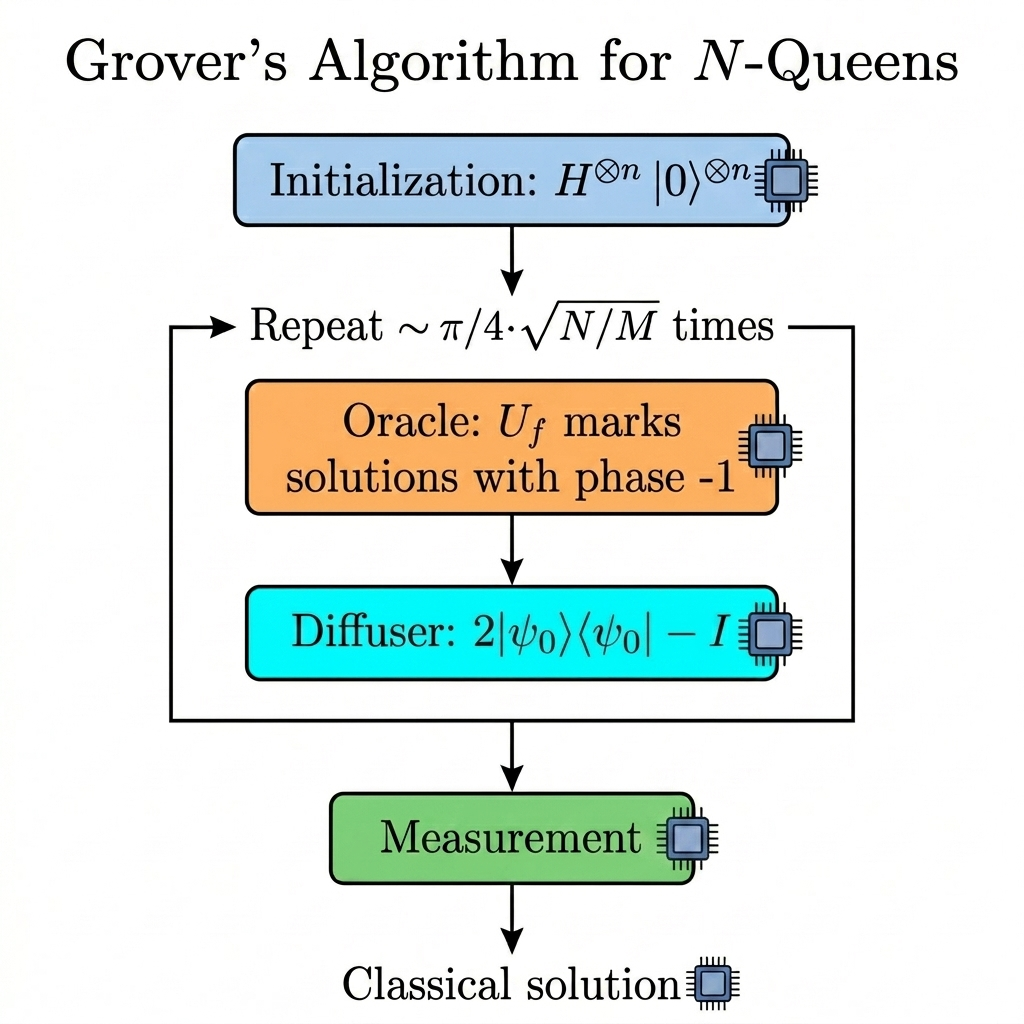
\includegraphics[width=0.72\columnwidth]{grover_high_level.png}
    \caption{Flow of Grover's algorithm for N-Queens.}
    \label{fig:high_level}
\end{figure}

\subsection{Geometric Interpretation}

The state of the system lives in a two-dimensional plane spanned by:
\begin{equation}
    \ket{\alpha} = \frac{1}{\sqrt{\mathcal{N}-M}} \sum_{f(x)=0} \ket{x},\quad
    \ket{\beta} = \frac{1}{\sqrt{M}} \sum_{f(x)=1} \ket{x}
\end{equation}
The initial state $\ket{\psi_0}$ forms an angle $\theta/2 = \arcsin\sqrt{M/\mathcal{N}}$
with $\ket{\alpha}$. Each iteration rotates the state by an angle $\theta$
towards $\ket{\beta}$.

\subsection{Optimal Iterations}

The optimal number of iterations is:
\begin{equation}
    t^* = \left\lfloor \frac{\pi}{2\theta} - \frac{1}{2} \right\rceil,\;\;
    \theta = 2\arcsin\!\sqrt{\frac{M}{\mathcal{N}}}
\end{equation}
For $N\!=\!4$: $\mathcal{N}\!=\!256$, $M\!=\!2$, $\theta \approx 0.177$~rad,
$t^*\!=\!8$, $P(\text{success})\!\approx\!99.6\%$.
\textbf{Note:} If $t^*$ is exceeded, the probability \emph{decreases}
--- the algorithm ``overshoots'' the solution.
This phenomenon has no classical analogue.
% ======================== 3. ENCODING ========================
\section{Quantum Encoding}

\subsection{Row Symmetry Elimination}

The first design decision is to implicitly fix each queen $i$ in row $i$.
This eliminates row conflicts by construction and reduces the search space
from $N^{2N}$ (arbitrary positions) to $N^N$ (only columns per queen).

\subsection{State Register}

The column of queen $i$ is encoded using $k = \lceil\log_2 N\rceil$ binary qubits.
The qubits $q_{ik}, q_{ik+1}, \ldots, q_{ik+k-1}$ represent the column in base 2,
with $q_{ik}$ as the least significant bit (LSB).
For $N\!=\!4$: $k\!=\!2$, total register of $n = Nk = 8$ qubits (Fig.~\ref{fig:encoding}).

\begin{figure}[H]
    \centering
    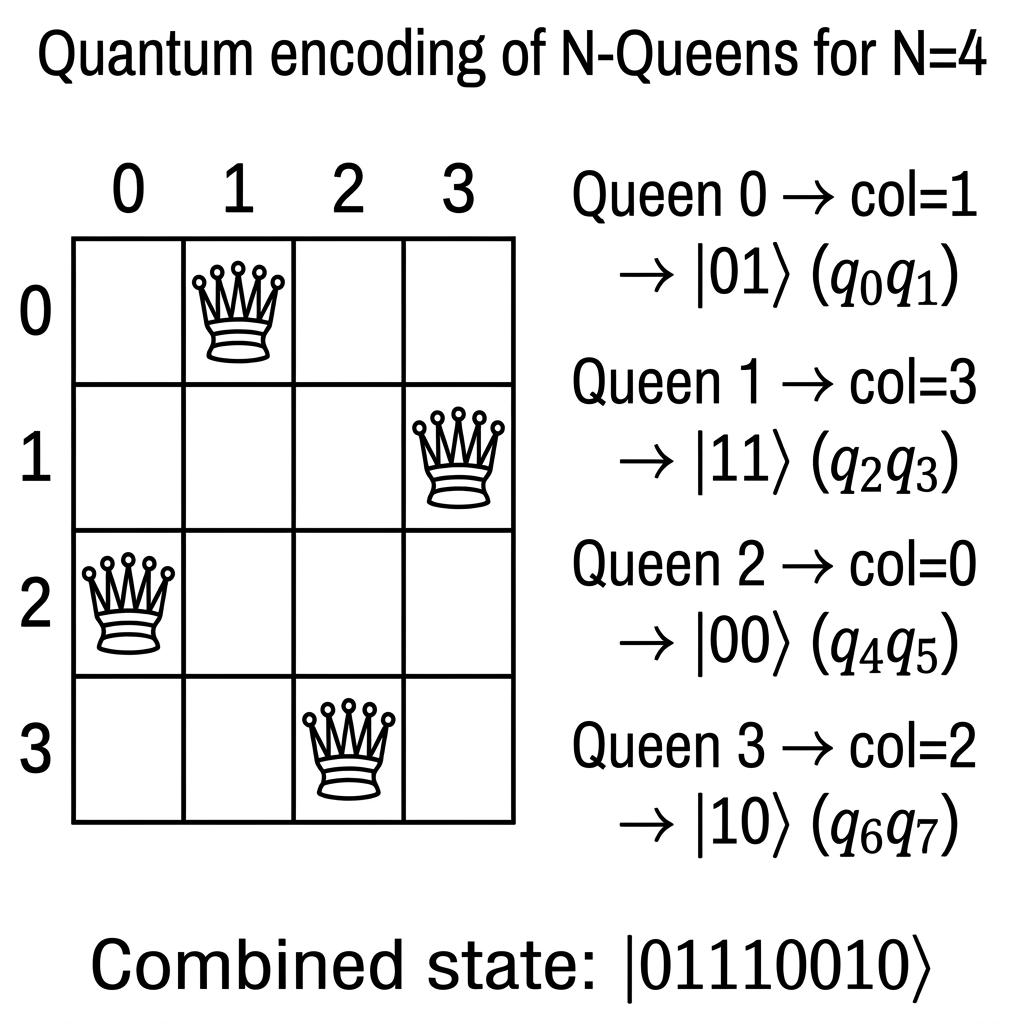
\includegraphics[width=0.72\columnwidth]{nqueens_encoding.png}
    \caption{Encoding of $[1,3,0,2]$ for $N=4$: 2 qubits per queen.}
    \label{fig:encoding}
\end{figure}

\subsection{Ancilla Qubits (Flags)}

The oracle requires auxiliary qubits:
\textbf{Pair flags}: one qubit for each pair $(i,j)$ with $i<j$, totaling
$\binom{N}{2}$ flags.
\textbf{Range flags} (only when $2^k > N$): one qubit per queen to detect columns
outside $[0, N)$. For $N\!=\!4$, $2^2 = 4 = N$, they are not needed; for $N\!=\!5$
($2^3 = 8 > 5$), 5 flags are added.

\begin{table}[H]
    \centering
    \caption{Circuit resources according to $N$.}
    \label{tab:resources}
    \small
    \renewcommand{\arraystretch}{1.3}
    \begin{tabular}{@{}ccccccc@{}}
        \toprule
        $N$ & $k$ & State & Pair flags & Range flags & Total & Sols. \\
        \midrule
        4 & 2 & 8  & 6  & 0 & 14 & 2  \\
        5 & 3 & 15 & 10 & 5 & 30 & 10 \\
        6 & 3 & 18 & 15 & 6 & 39 & 4  \\
        \bottomrule
    \end{tabular}
\end{table}

% ======================== 4. ORACLE ========================
\section{Oracle Design}

The oracle is the core component of the circuit. It applies a $-1$ phase exclusively
to states representing valid configurations, in three stages (Fig.~\ref{fig:oracle}):
\emph{compute}, \emph{phase flip}, and \emph{uncompute}.

\begin{figure}[H]
    \centering
    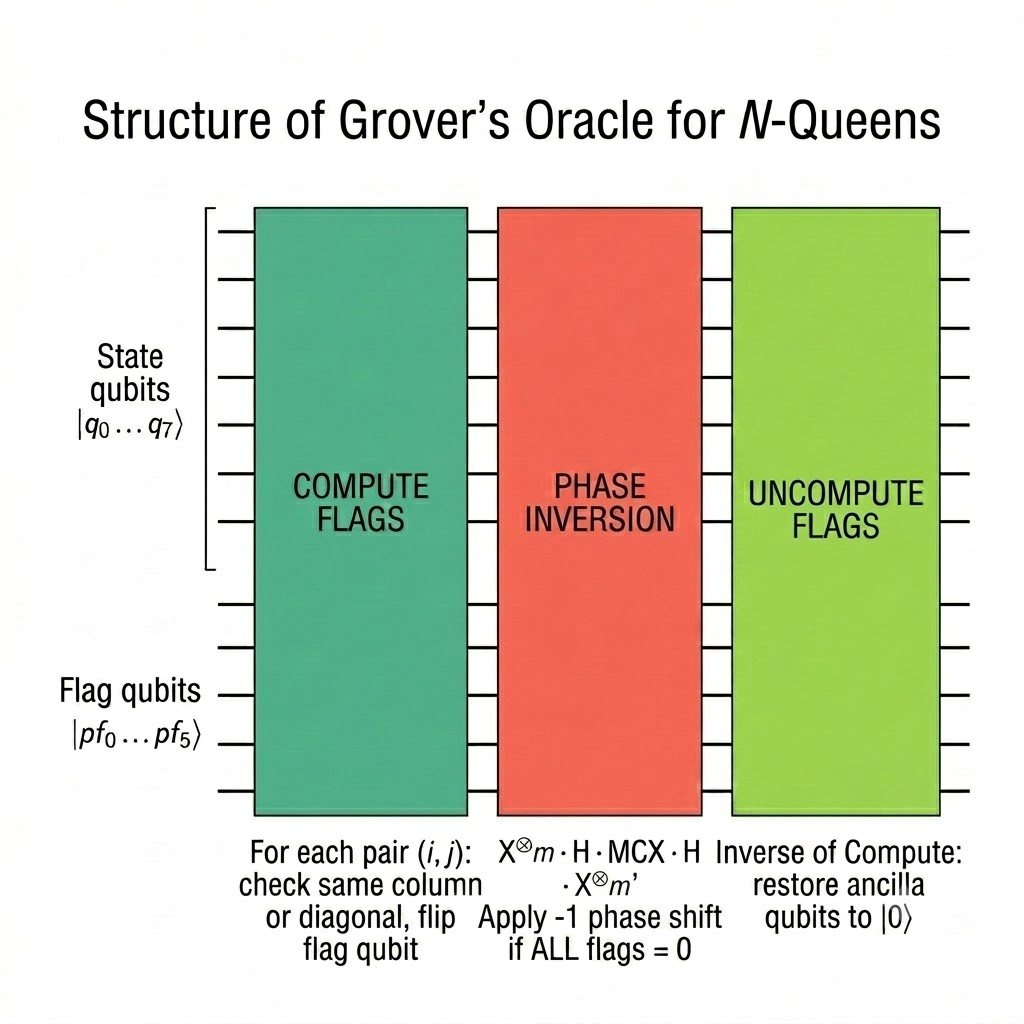
\includegraphics[width=0.85\columnwidth]{oracle_structure.png}
    \caption{Structure: Compute $\to$ Phase Flip $\to$ Uncompute.}
    \label{fig:oracle}
\end{figure}

\subsection{Compute Flags}

For each pair $(i, j)$, $i < j$, a conflict ($c_i = c_j$ or $|c_i - c_j| = j - i$)
is checked through \textbf{explicit pattern enumeration} (Fig.~\ref{fig:conflict}).

\vspace{0.2cm}
\noindent\textbf{Computational Cost:} This verification minimizes width by applying $X$ gates \textit{in-place}, but its depth scales as $\BigO(N^3 \log^2 N)$ due to the generalized Toffoli (MCX) gates required for pattern evaluation. This explains the massive resource cost for boards with $N \ge 5$.

\begin{figure}[H]
    \centering
    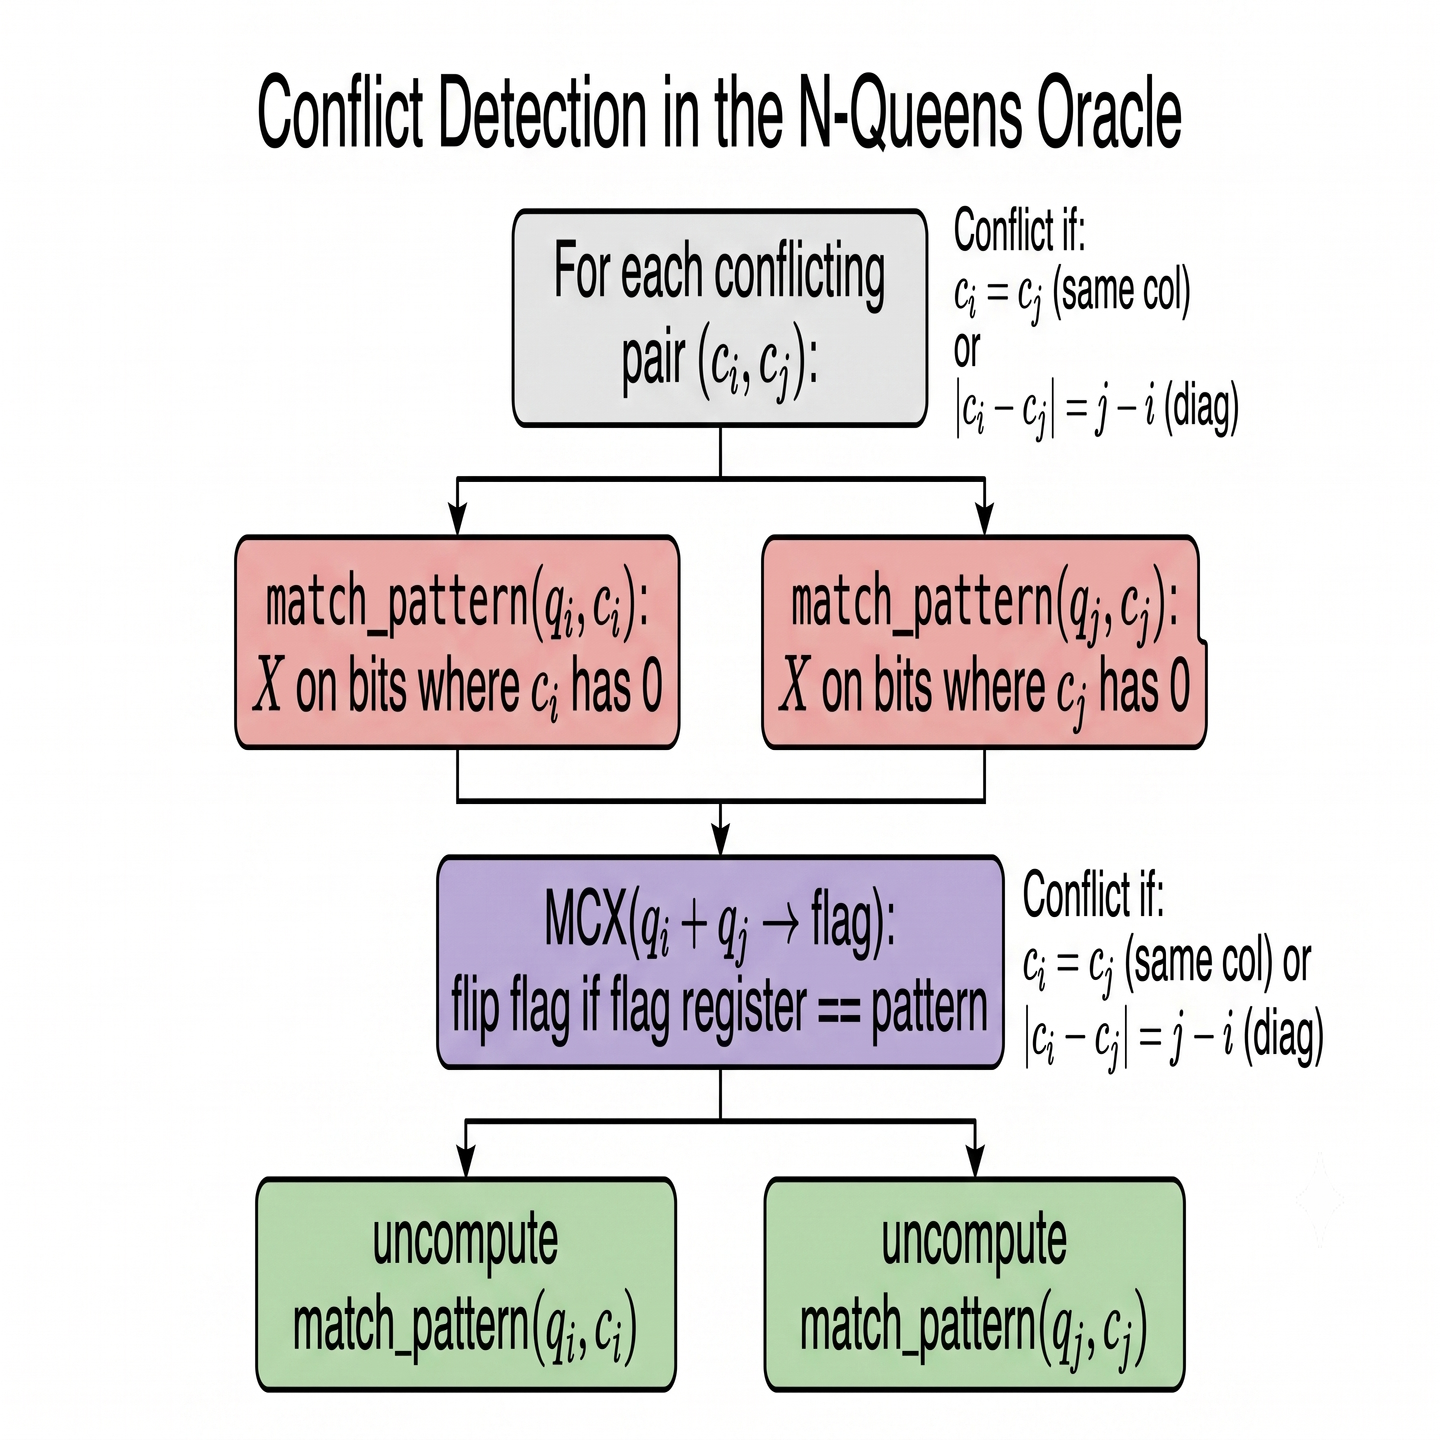
\includegraphics[width=0.85\columnwidth]{conflict_detection.png}
    \caption{Conflict detection $(c_i, c_j)$ with \texttt{match\_pattern}.}
    \label{fig:conflict}
\end{figure}

\subsubsection{Function match\_pattern}

This is the key piece for detection. Given a register of $k$ qubits and a target
value $v$, it applies $X$ gates to each qubit whose corresponding bit in $v$ is 0:
\begin{equation}
    \bigotimes_{b=0}^{k-1} X^{1-v_b} \ket{v} = \ket{1}^{\otimes k}
\end{equation}
This transforms the condition "the register equals $v$" into "all qubits equal 1",
which is exactly what an MCX (generalized Toffoli) gate detects. A subsequent MCX
flips the corresponding flag. Finally, the same sequence of $X$ is applied to restore
the register ($X^2 = I$).
For a fixed computational state $\ket{c_i, c_j}$, exactly one pattern combination
matches, guaranteeing that the flag is flipped 0 or 1 times.

\subsubsection{Out-of-Range Detection}

For $N$ that is not a power of 2 (e.g., $N = 5$ with $k = 3$), column values
$\{N, N{+}1, \ldots, 2^k{-}1\}$ are invalid. An additional flag per queen activates
if its column encodes a value $\geq N$, using the same \texttt{match\_pattern}
technique.

\subsection{Phase Flip}

Once all flags are computed, $-1$ is applied conditionally on all of them being 0
(no conflicts or out-of-range columns):
\begin{equation}
    X^{\otimes m}\!\cdot\!\big(H\!\cdot\!\text{MCX}\!\cdot\!H\big)\!\cdot\!X^{\otimes m}
\end{equation}
where $m$ is the total number of flags. The $X^{\otimes m}$ sequence converts
$\ket{0}^{\otimes m}$ into $\ket{1}^{\otimes m}$ (which triggers the MCX). The
$H \cdot \text{MCX} \cdot H$ trick implements an MCZ (controlled phase):
\begin{equation}
    HXH = Z \implies H \cdot \text{MCX}(\vec{c} \to t) \cdot H = \text{MCZ}(\vec{c}, t)
\end{equation}

\subsection{Uncompute Flags}

For the oracle to be unitary and reusable between iterations, ancillas must return
to $\ket{0}$. The Compute stage is undone by applying the same operations in reverse
order. Since $X$ and MCX are self-inverses, this inversion is straightforward.

\vspace{0.3cm}
\noindent
\colorbox{boxbg}{%
\begin{minipage}{\dimexpr\columnwidth-2\fboxsep\relax}
\vspace{2pt}
{\small\sffamily\bfseries\color{accent} ENCODING COMPARISON}\par\vspace{1pt}
{\small\itshape
Unlike formulations based on special-purpose quantum simulators
with atoms in optical lattices~\cite{torggler2019}, and spatial mappings that use $N^2$
qubits by assigning one to each square~\cite{jha2018, santhosh2023},
the column encoding approach presented here requires only
$N \lceil\log_2 N\rceil$ state qubits. Although this drastically reduces
the required Hilbert space and guarantees by construction the absence
of row conflicts, it comes at the cost of a deeper decision oracle
to resolve the remaining combinatorial constraints.
}
\vspace{2pt}
\end{minipage}}
\vspace{0.3cm}

% ======================== 5. DIFFUSER ========================
\section{Grover's Diffuser}

It implements the reflection $D = 2\ket{\psi_0}\!\bra{\psi_0} - I$ (inversion about
the mean) on the $n$ state qubits. Its decomposition into gates is:
\begin{equation}
    D = H^{\otimes n}\!\cdot\!X^{\otimes n}\!\cdot\!\text{MCZ}
        \!\cdot\!X^{\otimes n}\!\cdot\!H^{\otimes n}
\end{equation}
The circuit (Fig.~\ref{fig:diffuser}) operates by: (1)~switching to the Hadamard
basis with $H^{\otimes n}$; (2)~marking $\ket{0\ldots 0}$ with $X^{\otimes n}$
followed by MCZ; (3)~undoing $X^{\otimes n}$ and returning to the computational basis.

\begin{figure}[H]
    \centering
    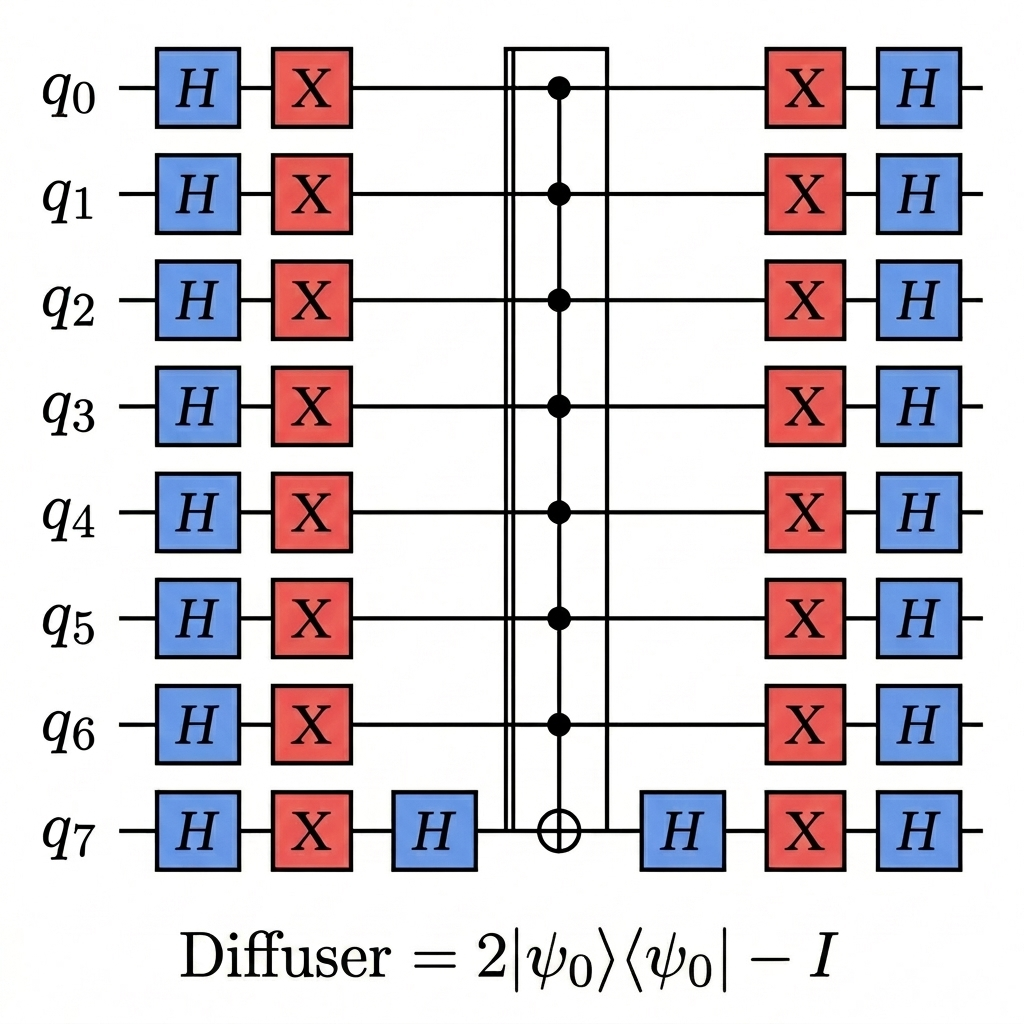
\includegraphics[width=0.68\columnwidth]{diffuser_circuit.png}
    \caption{Diffuser circuit for 8 state qubits.}
    \label{fig:diffuser}
\end{figure}

\noindent\textbf{Effect on amplitudes.} Let $\bar{a}$ be the mean amplitude. The
diffuser transforms each amplitude $a_x \to 2\bar{a} - a_x$: states with amplitude
below the mean are attenuated, while solutions (with large negative amplitude) are
reflected to large positive values.

% ======================== 6. RESULTS ========================
\section{Results}

\subsection{\texorpdfstring{$N=4$}{N=4}: Full Execution}

For $N = 4$, the complete circuit was simulated with the \texttt{AerSimulator}
backend (\texttt{statevector} method) for 4096 shots.

\begin{table}[H]
    \centering
    \caption{Circuit parameters for $N = 4$.}
    \label{tab:params}
    \scriptsize
    \begin{tabular}{@{}ll@{}}
        \toprule
        Parameter & Value \\
        \midrule
        State qubits & 8 (2 bits/column) \\
        Pair flags & 6 \\
        Total qubits & 14 \\
        Search space & $2^8 = 256$ \\
        Classical solutions & 2 \\
        Optimal iterations & 8 \\
        Depth (transpiled) & $\sim$41\,000 \\
        \bottomrule
    \end{tabular}
\end{table}

The two valid solutions, $[1,3,0,2]$ and $[2,0,3,1]$, concentrate $\sim\!99.6\%$
of the total probability ($\sim$49.6\% each, Fig.~\ref{fig:results}).
Decoding the measured bitstring is done by reversing the bit order (Qiskit prints
MSB first) and reconstructing each queen's column:
$\text{col}_i = \sum_{b=0}^{k-1} c_{ik+b} \cdot 2^b$.

\begin{figure}[H]
    \centering
    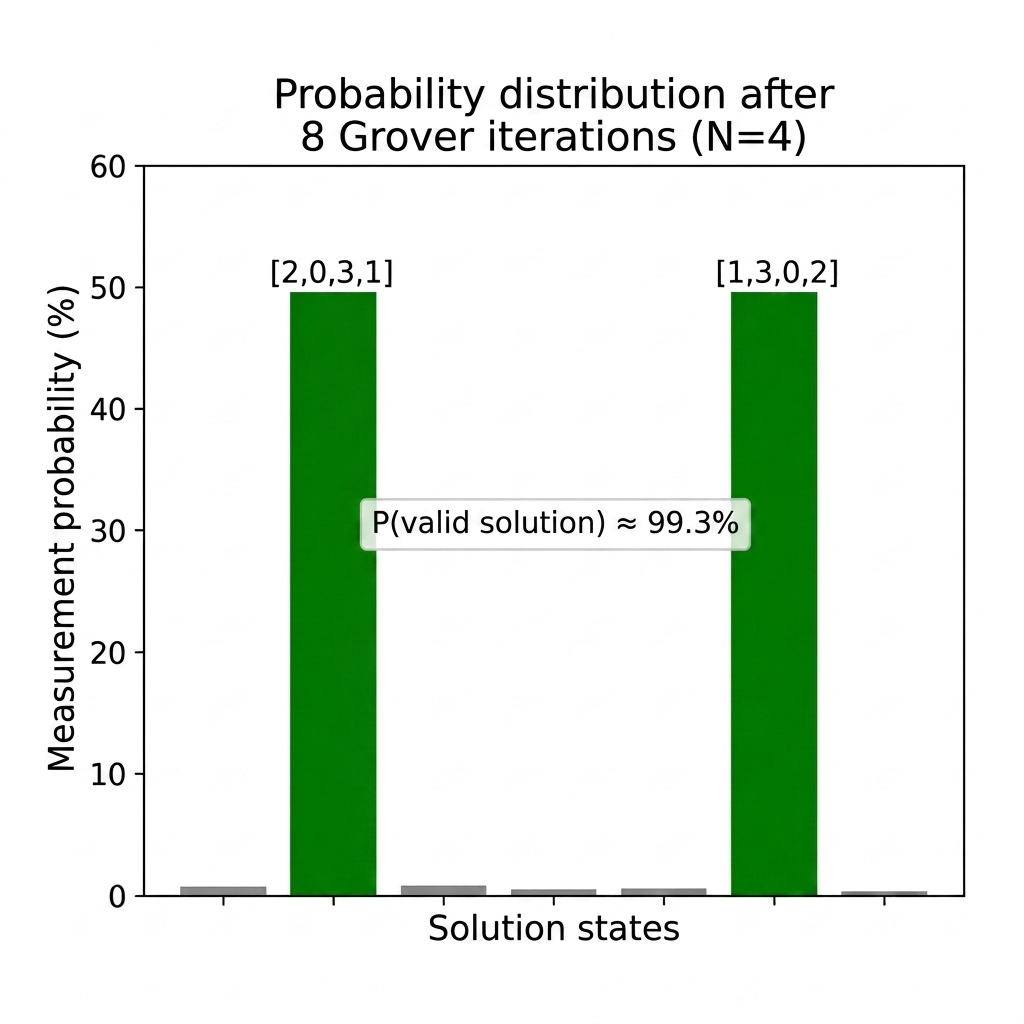
\includegraphics[width=0.78\columnwidth]{measurement_results.png}
    \caption{Probability after 8 iterations ($N\!=\!4$). The two solutions
    dominate with $\sim$49.6\% each; noise $<1\%$.}
    \label{fig:results}
\end{figure}

\subsection{\texorpdfstring{$N=5$}{N=5}: Oracle Validation}

The complete circuit for $N\!=\!5$ requires 30 qubits and $\sim$44 iterations
($\sim\!6\!\times\!10^5$ gates), which is beyond the practical reach of classical
simulation. However, the oracle was validated in isolation by preparing known
computational states and measuring the flags:

The \textbf{10 classical solutions} (obtained via brute force with
\texttt{classical\_solutions}) resulted in 0 active flags in all cases.
Tested negative cases included:
\columnbreak
\begin{itemize}
    \item $[0,0,0,0,0]$: all in the same column.
    \item $[0,1,2,3,4]$: main diagonal.
    \item $[0,2,4,1,7]$: column 7 out of range ($\geq 5$).
    \item $[1,3,5,0,2]$: column 5 out of range.
\end{itemize}
All were correctly rejected with flags $> 0$. This confirms that the oracle
perfectly separates valid configurations from the rest of the search space.

% ======================== 7. COMPLEXITY ========================
\section{Complexity and Limitations}

\subsection{Oracle Complexity}

Explicit pattern enumeration yields:
$\binom{N}{2} = \BigO(N^2)$ pairs of queens;
up to $\BigO(N)$ conflicting combinations per pair;
each check: $\BigO(k)$ $X$ gates plus an MCX with $2k$ controls.
Total: $\BigO(N^3)$ MCX calls and $\BigO(N^3 \log N)$ elementary gates.
An implementation using \textbf{quantum adders} would allow for arithmetic column
comparisons, reducing MCX gates per pair from $\BigO(N)$ to $\BigO(\text{poly}(k))$.

\subsection{Scalability}

\begin{table}[H]
    \centering
    \caption{Simulation feasibility according to $N$.}
    \label{tab:scale}
    \scriptsize
    \begin{tabular}{@{}cccl@{}}
        \toprule
        $N$ & Qubits & Iters. & Simulable \\
        \midrule
        4 & 14 & 8    & Yes (\texttt{statevector}) \\
        5 & 30 & 44   & Oracle only (\texttt{MPS}) \\
        6 & 39 & $\sim$200 & No (classical simulator) \\
        \bottomrule
    \end{tabular}
\end{table}

For $N \geq 5$, the two paths to end-to-end execution are:
(1)~real quantum hardware with sufficient fidelity and $T_1/T_2$
(aspirational in 2026); or (2)~rewriting the oracle with quantum adders to
reduce circuit depth.

% ======================== 8. CONCLUSIONS ========================
\section{Conclusions}

\begin{enumerate}
    \item \textbf{Verified Correctness.}
          For $N\!=\!4$, the full algorithm finds the 2 solutions with $P \approx 99.6\%$.
          For $N\!=\!5$, the oracle correctly classifies the 10 solutions and rejects
          all tested invalid cases.

    \item \textbf{Quadratic Speedup.}
          The algorithm queries the oracle $\BigO\!\big(\sqrt{\mathcal{N}/M}\big)$ times,
          compared to $\BigO(\mathcal{N}/M)$ in classical search.
          For $N\!=\!4$: 8 iterations vs.\ $\sim$128 classical queries.

    \item \textbf{Modular Design.}
          The separation into encoding, oracle (compute--phase--uncompute), and
          diffuser allows for independent extension or replacement of components.

    \item \textbf{Main Limitation.}
          Explicit enumeration generates deep circuits ($\sim$41\,000 depth for $N\!=\!4$).
          Quantum adders would significantly reduce the depth for $N\!\geq\!5$.

    \item \textbf{Perspective.}
          Execution on real quantum hardware would require coherence times ($T_1$, $T_2$)
          vastly superior to those currently available, along with quantum error
          correction. Nevertheless, this implementation serves as a conceptual
          demonstration of Grover's quadratic advantage on combinatorial problems.
\end{enumerate}

% ======================== BIBLIOGRAPHY ========================
\begin{thebibliography}{9}
\small
    \bibitem{grover1996}
    L.\,K.~Grover,
    ``\href{https://doi.org/10.1145/237814.237866}{A fast quantum mechanical algorithm for database search},''
    \textit{Proc.\ 28th ACM STOC}, pp.\,212--219, 1996.

    \bibitem{nielsen2010}
    M.\,A.~Nielsen and I.\,L.~Chuang,
    \href{https://doi.org/10.1017/CBO9780511976667}{\textit{Quantum Computation and Quantum Information}},
    Cambridge Univ.\ Press, 10th Ann.\ Ed., 2010.

    \bibitem{qiskit}
    Qiskit Development Team,
    ``\href{https://qiskit.org}{Qiskit: An open-source framework for quantum computing},''
    2024.

    \bibitem{nqueens}
    J.~Bell and B.~Stevens,
    ``\href{https://doi.org/10.1016/j.disc.2007.12.043}{A survey of known results and research areas for $n$-queens},''
    \textit{Discrete Math.}, vol.\,309, no.\,1, pp.\,1--31, 2009.

    \bibitem{bennett1997}
    C.\,H.~Bennett, E.~Bernstein, G.~Brassard, and U.~Vazirani,
    ``\href{https://doi.org/10.1137/S0097539796300933}{Strengths and weaknesses of quantum computing},''
    \textit{SIAM J.\ Comput.}, vol.\,26, no.\,5, pp.\,1510--1523, 1997.

    \bibitem{jha2018}
    R.~Jha, D.~Das, A.~Dash, S.~Jayaraman, B.\,K.~Behera, and P.\,K.~Panigrahi,
    ``\href{https://arxiv.org/abs/1806.10221}{A novel quantum N-queens solver algorithm and its simulation
    and application to satellite communication using IBM Quantum Experience},''
    arXiv:1806.10221 [quant-ph], 2018.

    \bibitem{santhosh2023}
    S.\,G.\,S.~Santhosh, P.~Joshi, A.~Barui, and P.\,K.~Panigrahi,
    ``\href{https://arxiv.org/abs/2312.16312}{A quantum approach to solve N-queens problem},''
    arXiv:2312.16312 [quant-ph], 2023.

    \bibitem{torggler2019}
    V.~Torggler, P.~Aumann, H.~Ritsch, and W.~Lechner,
    ``\href{https://doi.org/10.22331/q-2019-06-03-149}{A quantum N-queens solver},''
    \textit{Quantum}, vol.\,3, p.\,149, 2019.
    arXiv:1803.00735 [quant-ph].
\end{thebibliography}

\end{multicols}

\end{document}
